
\newcommand{\cia}{\begin{figure}[H]
\centering
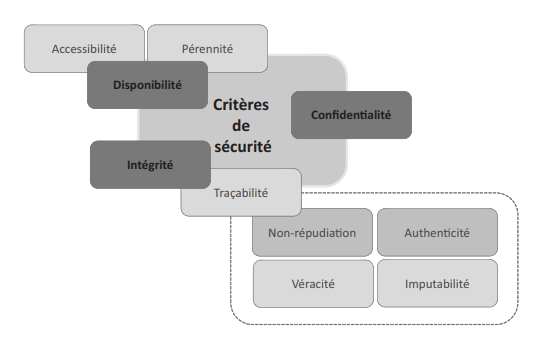
\includegraphics{images/CIA}
\caption{Critères de sécurité informatique \cite{ref4}}
\label{imagecia}
\end{figure}
}

\newcommand{\dl}{\begin{figure}[H]
\centering
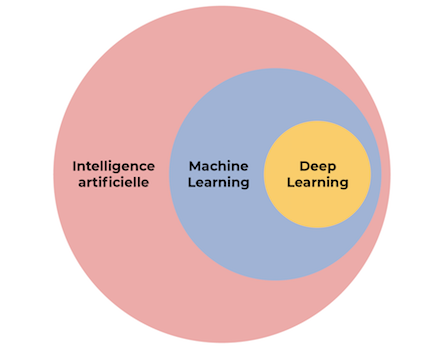
\includegraphics[height=5cm]{images/dl}
\caption{Position du Deep Learning dans l'IA \cite{refclassroom}}
\label{dl}
\end{figure}
}

\newcommand{\nslkdd}{\begin{figure}[H]
\centering
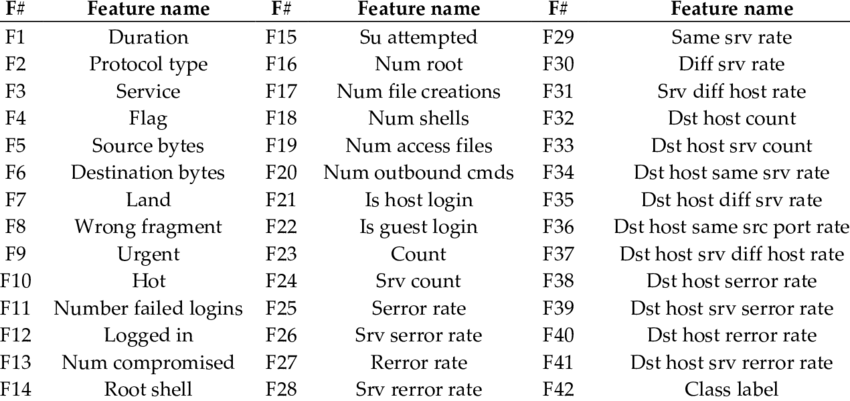
\includegraphics[width=\textwidth]{images/nslkdd}
\caption{Liste des caractéristiques de NSL-KDD. \cite{kdd}}
\label{nslkdd}
\end{figure}
}
\newcommand{\architecture}{\begin{figure}[H]
\centering
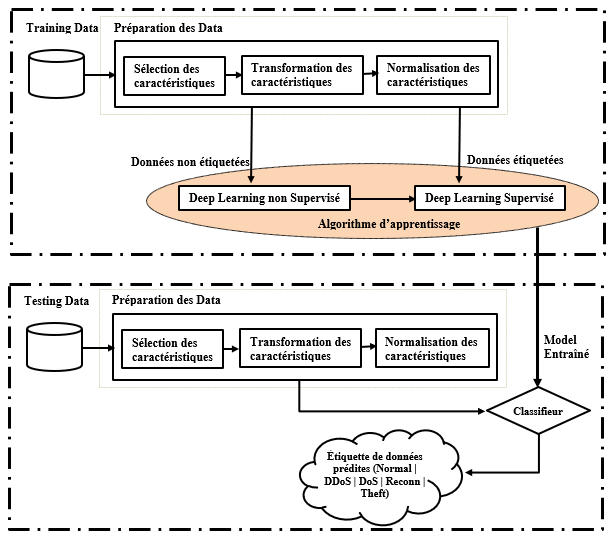
\includegraphics[width=\textwidth]{images/architecture}
\caption{L'architecture de notre approche }
\label{architecture}
\end{figure}
}
\newcommand{\modelAE}{\begin{figure}[H]
\centering
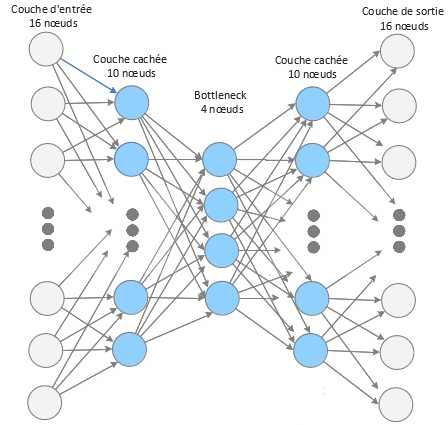
\includegraphics[width=\textwidth]{images/ModelAE}
\caption{Structure de l'AE}
\label{modelAE}
\end{figure}
}
\newcommand{\modelDNN}{\begin{figure}[H]
\centering
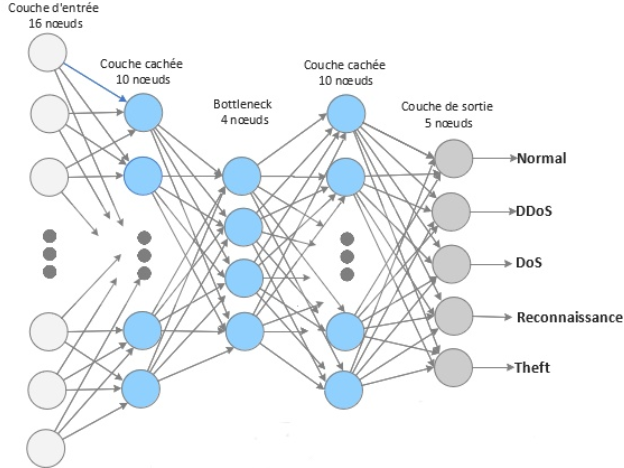
\includegraphics[width=\textwidth]{images/ModelDNN}
\caption{Structure du DNN}
\label{modelDNN}
\end{figure}
}
\newcommand{\iot}{\begin{figure}[H]
\centering
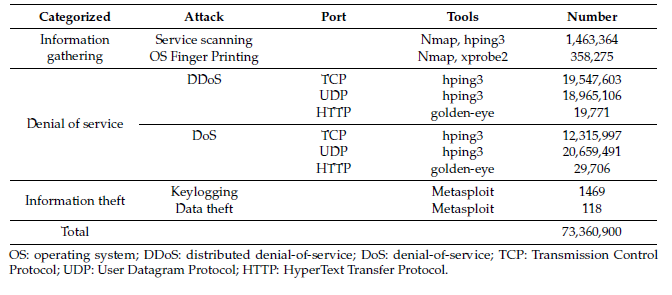
\includegraphics[width=\textwidth]{images/iot}
\caption{Résumé des attaques du Dataset Iot Botnet \cite{kdd}}
\label{nslkdd}
\end{figure}
}
%%%%%%%%%%%%%%%%%%%%%%%%%%%%%%%%%%%

\newcommand{\source}[1]{\caption*{ {#1}} 
}
%\source{\cite{ref4}}

\newcommand{\imageAPS}{\begin{figure}[!h]
\centering
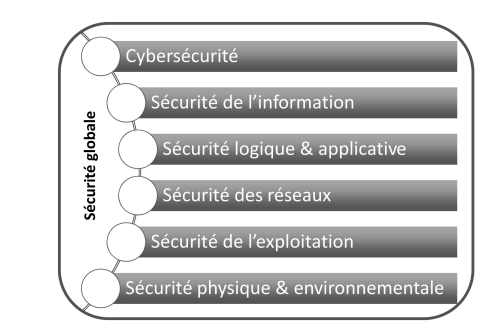
\includegraphics{images/applicationsécurité}
\caption{Application de sécurité informatique \cite{ref4}}
\label{imagecia}
\end{figure}
}

\newcommand{\imgMiM}{\begin{figure}[H]
\centering
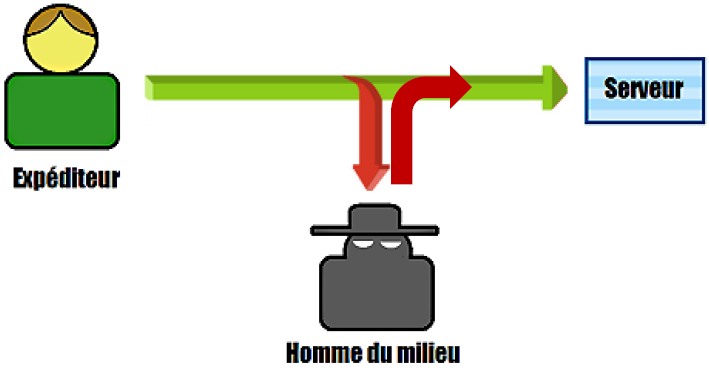
\includegraphics[width=\textwidth]{images/MiM}
\caption{main-in-the-middle}
\label{imagMiM}
\end{figure}
}
\newcommand{\typedl}{\begin{figure}[H]
\centering
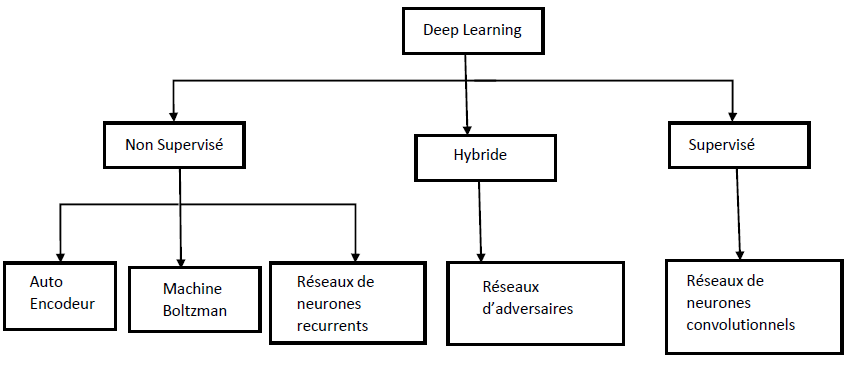
\includegraphics[width=\textwidth]{images/typedl}
\caption{classification des modèles de deep learning}
\label{typedl}
\end{figure}
}

\newcommand{\cnn}{\begin{figure}[H]
\centering
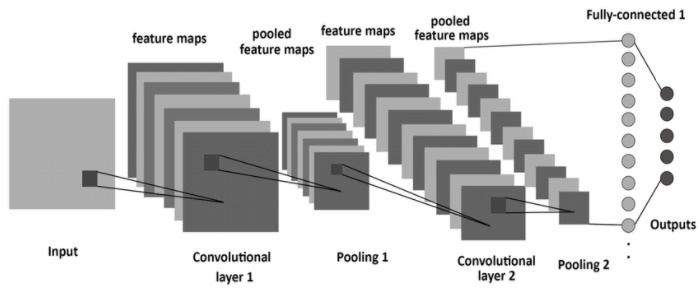
\includegraphics[width=\textwidth]{images/cnn}
\caption{Architecture classique d’un réseau de neurones convolutif \cite{cnn}}
\label{cnn}
\end{figure}
}

\newcommand{\autoencodeur}{\begin{figure}[H]
\centering
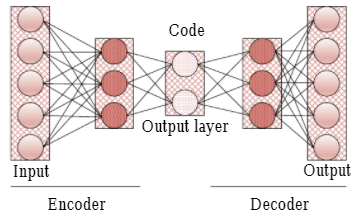
\includegraphics[width=\textwidth]{images/autoencodeur}
\caption{Architecture Auto Encodeur\cite{autoencodeur}}
\label{autoencodeur}
\end{figure}
}

\newcommand{\perceptron}{\begin{figure}[!h]
\centering
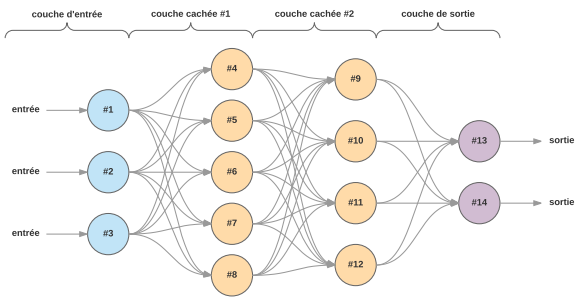
\includegraphics[width=\textwidth]{images/perceptron}
\caption{Réseau de neurone profond (DNN)}
\label{perceptron}
\end{figure}
}

\newcommand{\graphe}{\begin{figure}[H]
\centering
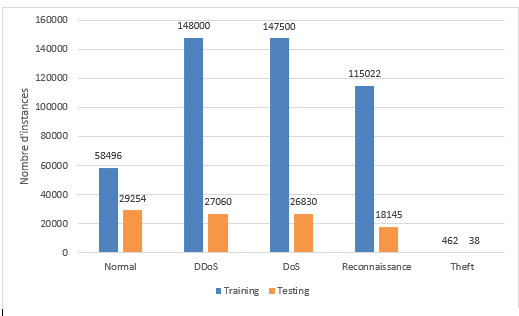
\includegraphics[width=\textwidth]{images/graphe}
\caption{Nombres d'éléments par types de datasets}
\label{graphe}
\end{figure}
}

\newcommand{\neurone}{\begin{figure}[H]
\centering
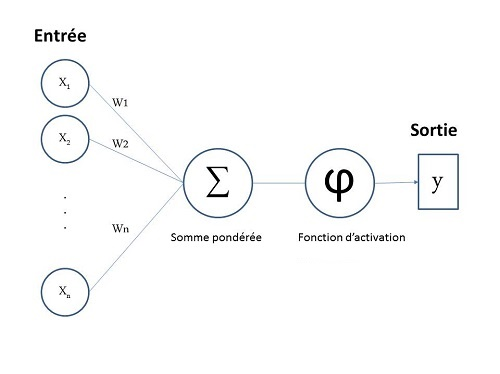
\includegraphics[height=7cm]{images/neuroneF}
\caption{Représentation d'un neurone formel}
\label{atnn}
\end{figure}
}

\newcommand{\cidf}{\begin{figure}[H]
\centering
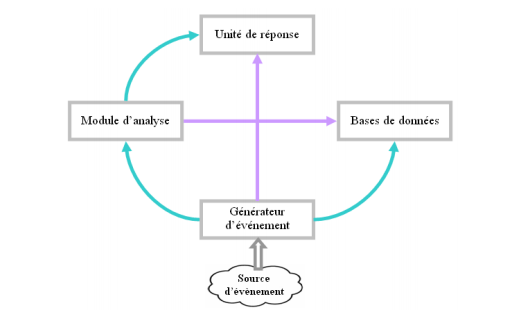
\includegraphics[width=\textwidth]{images/icef}
\caption{l’architecture CIDF \cite{zaidi}}
\label{imagMiM}
\end{figure}
}

\newcommand{\apprentissage}{\begin{figure}[H]
\centering
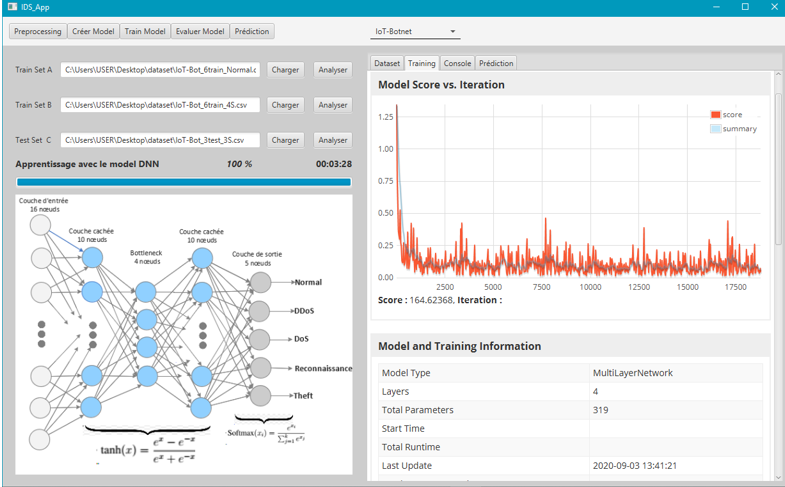
\includegraphics[width=\textwidth]{images/apprentissage}
\caption{Entrainement du modèle DNN}
\label{apprentisage}
\end{figure}
}

\newcommand{\prediction}{\begin{figure}[H]
\centering
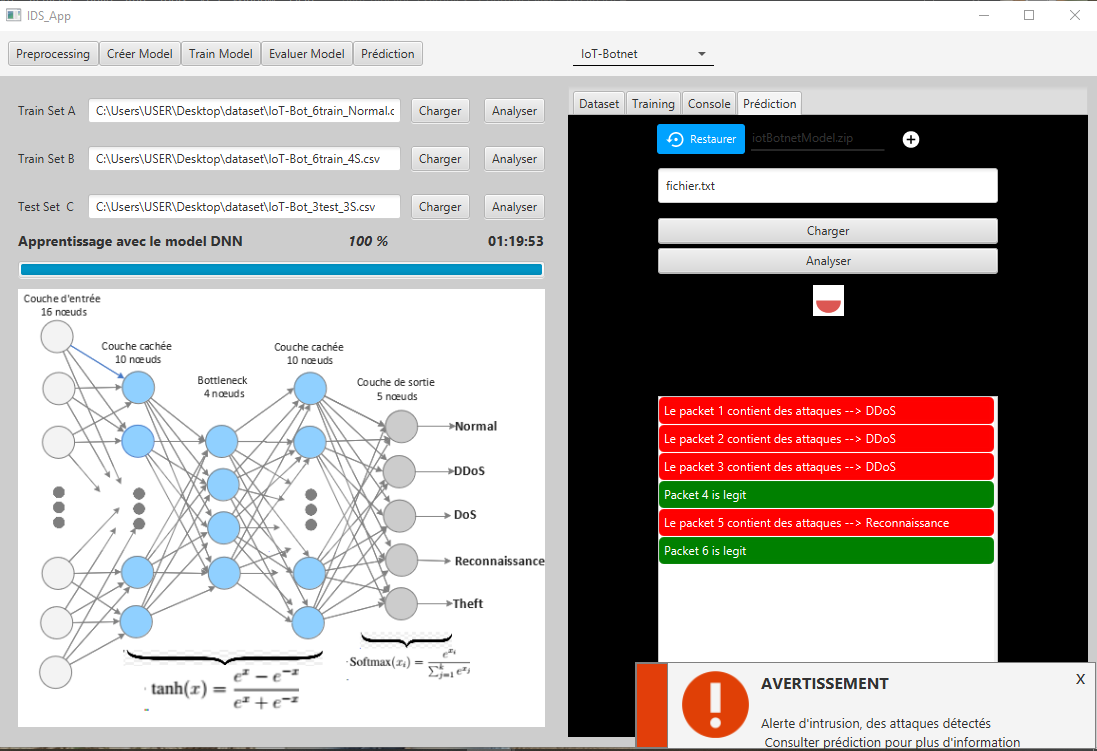
\includegraphics[width=\textwidth]{images/predi}
\caption{prédiction d'attaques}
\label{apprentisage}
\end{figure}
}

\newcommand{\data}{\begin{figure}[H]
\centering
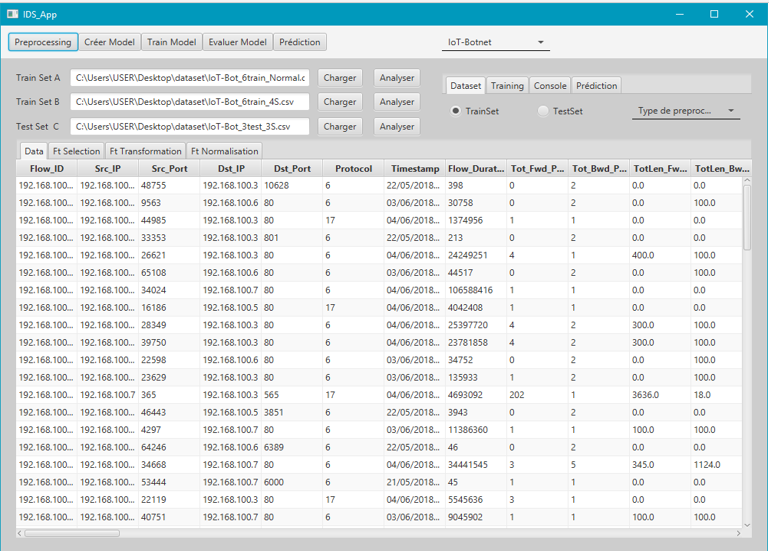
\includegraphics[width=\textwidth]{images/data}
\caption{structure du dataset}
\label{data}
\end{figure}
}

\newcommand{\analyse}{\begin{figure}[H]
\centering
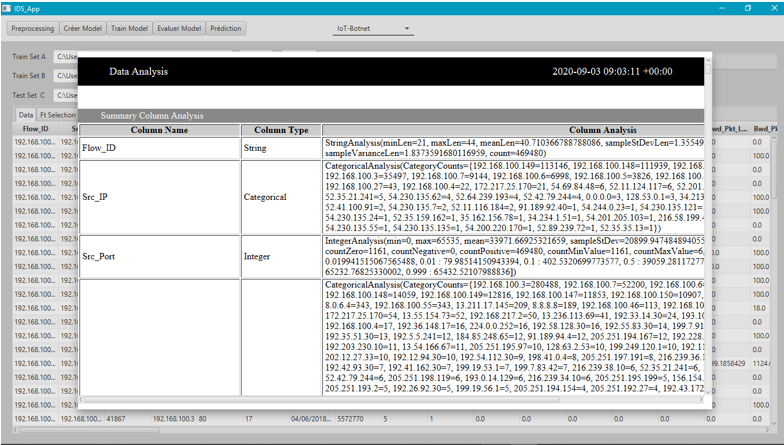
\includegraphics[width=\textwidth]{images/dataanalyse}
\caption{Analyse des données}
\label{data}
\end{figure}
}

\newcommand{\evaluation}{\begin{figure}[H]
\centering
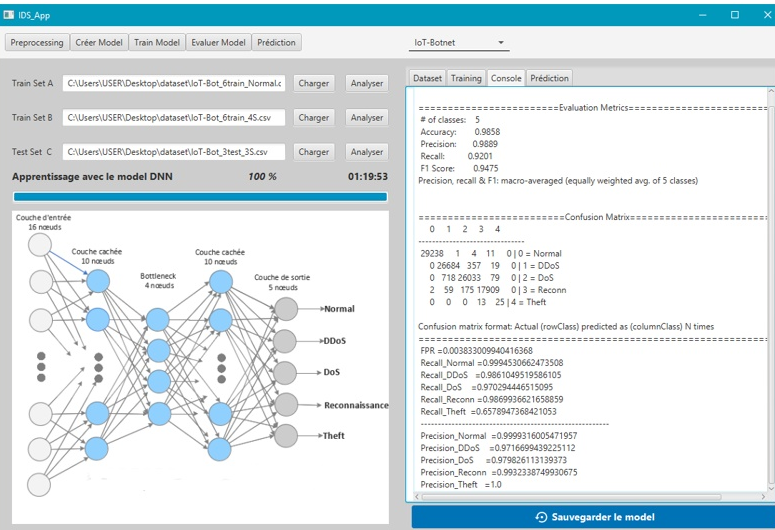
\includegraphics[width=\textwidth]{images/evaluation}
\caption{Evaluation du modèle}
\label{apprentisage}
\end{figure}
}
\newcommand{\idwg}{\begin{figure}[H]
\centering
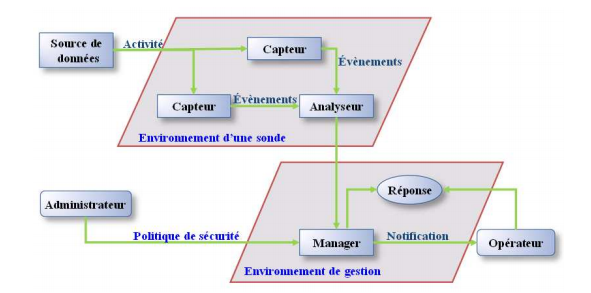
\includegraphics[width=\textwidth]{images/IDWG}
\caption{L’architecture IDWG \cite{zaidi}}
\label{idwg}
\end{figure}
}
\newcommand{\typeids}{\begin{figure}[H]
\centering
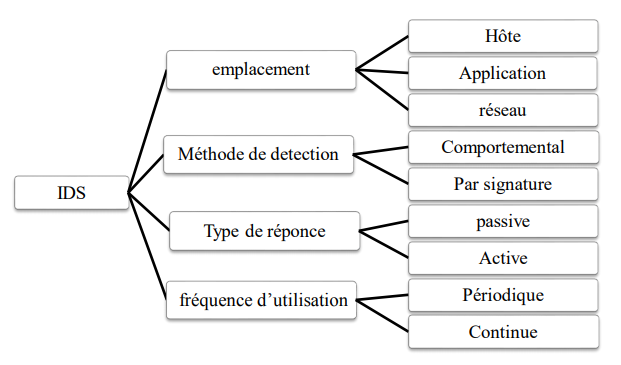
\includegraphics[width=\textwidth]{images/ids}
\caption{Classification des différents types d'IDS  \cite{reftypeids}}
\label{ids}
\end{figure}
}
\newcommand{\hids}{\begin{figure}[H]
\centering
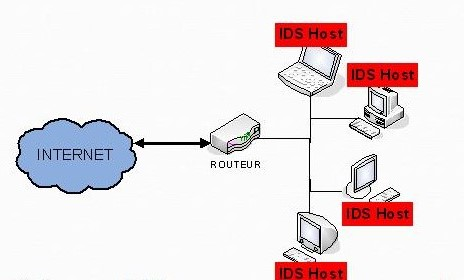
\includegraphics[width=\textwidth,height=10cm]{images/HIDS}
\caption{La détection d'intrusion basée sur l'hôte \cite{refphototypids}}
\label{hids}
\end{figure}
}
\newcommand{\nids}{\begin{figure}[H]
\centering
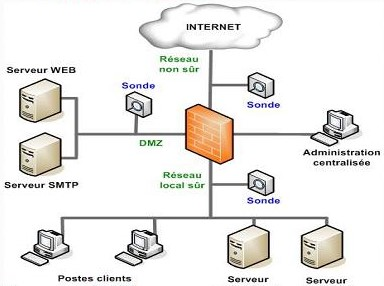
\includegraphics[width=\textwidth,height=10cm]{images/NIDS}
\caption{La Détection d'Intrusion Réseau (NIDS) \cite{refphototypids}}
\label{nids}
\end{figure}
}

\newcommand{\authenti}{\begin{figure}[H]
\centering
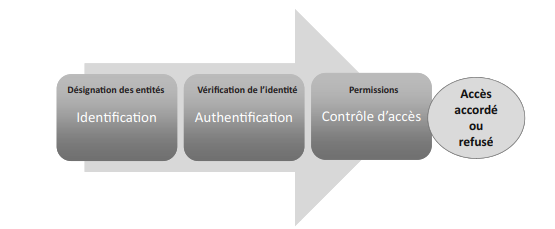
\includegraphics{images/authentification}
\caption{Accès à une ressource \cite{ref4}}
\label{Authentification}
\end{figure}
}

\newcommand{\ransom}{\begin{figure}[H]
\centering
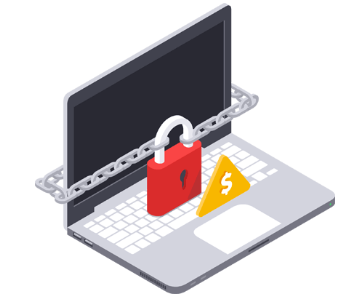
\includegraphics{images/ransomware}
\caption{Ransomware}
\label{ransomware}
\end{figure}
}


\newcommand{\logoucd}{\begin{figure}[!h]
\centering

\includegraphics[width=0.2\linewidth]{Images/Logo.png}
\label{logo}
\end{figure}
}
\newcommand{\pagedegarde}{
\begin{titlepage}
\newgeometry{top=1.5cm, bottom=1.5cm, left=2cm, right=1cm}
\AddToShipoutPicture*{\EtiquetteThese}
\begin{center}
\begin{minipage}{1\textwidth}
	\begin{center}
		\large\ministere{}
	\end{center}				
\end{minipage}
\vspace{0.9mm}
\logoucd\\
% \Huge{\emph{{{\it {Faculté des Sciences}}}}}\\
\normalsize
\begin{center}
 \huge{\textbf{MEMOIRE DE MASTER}}\\
 \vspace{1cm}
 \large{Domaine: Math et Informatique\\Département: Informatique\\
 Specialité: Informatique fondamentale et intelligence artificielle}
\end{center}

\vspace{1cm}
\Huge\textbf{Thème}
\noindent\rule{\textwidth}{0.9mm}
%\noindent\color{blueforest}\rule{\textwidth}{0.1mm}
\Large{\textbf{Classification hybride (Hard et Soft) d'items éducatifs similaires}}
%\noindent\color{blueforest}\rule{\textwidth}{0.1mm}
\noindent\rule{\textwidth}{0.9mm}
\end{center}
\vspace{1.5cm}
\begin{tabular}{l r}
\hspace{1cm}\textbf{Présenté par :}&\hspace{5cm}\textbf{Encadré par :}\\
\hspace{1cm}\textbf{\textcolor{blue}{Abdou Abarchi Aboubacar}}&\textbf{\textcolor{blue}{$M^{eme}$ Harbouche Khadidja}}\\
\end{tabular}
\vspace{2cm}
\begin{center}
\textbf{Juillet 2021}
\end{center}
\end{titlepage}
\restoregeometry  
\nopagebreak
}
\newcommand{\firstpart}{\part{\'Etat de l'art}}
\newcommand{\secondpart}{\part{Contributions}}
\newcommand{\ministere}{\textbf{R\'{e}publique  Alg\'{e}rienne D\'{e}mocratique et Populaire\\Ministère de  l'Enseignement Sup\'{e}rieur et de la Recherche Scientifique\\Université Ferhat Abbas Sétif 1\\Faculté des Sciences}}
\definecolor{blueforest}{RGB}{80,00,00}
\newcommand\EtiquetteThese{%
	\put(-10,10){%
		\parbox[t][\paperheight]{\paperwidth}{%
			\hfill
			\colorbox{blueforest}{		
				\begin{minipage}[b]{3em}
				\vspace{0.1cm}
					\centering\Huge\textcolor{white}{\textbf{M}\\\textbf{A}\\\textbf{S}\\\textbf{T}\\\textbf{E}\\\textbf{ R}}
					\vspace{0.2cm}
				\end{minipage}
			}
		}
	}
}



